\chapter{Implementation}
\label{chap:implementation}

After introducing the conceptual design and architecture of \texttt{Protego}, this chapter introduces an implementation of the system. Section \ref{sec:implementation-technology} discusses the main technological components used for the implementation. Section \ref{sec:implementation-core} presents the internals of the implementation of \texttt{Protego}. Finally, Section \ref{sec:implementation-poc} shows how to perform the activies needed with this implementation.

\section{Selected Technologies}
\label{sec:implementation-technology}

\subsection{Hyperledger Sawtooth}

The basis of the implementation will be a project named Hyperledger Sawtooth. Hyperledger Sawtooth is an open-source effort from The Linux Foundation \footnote{https://www.linuxfoundation.org/}, that introduces a modular platform for implementation of applications on top of permissioned distributed ledgers. We use it as the backbone of our implementation. As explained earlier, our approach needs to have a permissioned decentralized ledger, which needs to be customized, to be suitable for our purposes. Hyperledger Sawtooth offers a complete set of tools to build applications on top of a distributed ledger that include: REST API, a validator network infrastructure, permissioning capabilities, events, a consensus protocol - \gls{poet} - and, of course, a distributed ledger. To connect all the pieces together it offers \gls{sdk}, in a variety of languages such as Go, Python or Javascript, easing the development of the implementation. Other projects exist, such as Hyperledger Fabric, offering a wide array of different features, which don't quite suit our approach - such as \textit{smart contracts}.

\subsection{Python}

The implementation of \texttt{Protego} has been developed with the Python\footnote{https://www.python.org/} programming language. Specifically, the implementation only supports Python 3. Python is a dynamically typed, general-purpose programming language widely popular in software development. It has an established mature community, with a lot of resources available. Furthermore, Hyperledger Sawtooth provides 3 mature \gls{sdk} - Python, Go\footnote{https://golang.org/} and Javascript\footnote{https://nodejs.org/en/}. From those 3, only Python and Go had a mature Transaction Processor API. Given that situation, Python gives us more flexibility during development, being interpreted rather than compiled, while also providing us with a mature standard library, given it has a leaf of almost 20 years in development when compared with Go.

\subsection{Docker}

Docker is a platform for container execution. Setting up all the components that are needed to run the system can be complex. Hyperledger Sawtooth supports Docker files to help with configuration and execution of all the components at the same time. With that context, we used Docker in order to run containers of the Hyperledger Sawtooth infrastructure, in which we could our implementation against. This also eases setting up because it doesn't modify any part of the user's system.

\section{Implementation}
\label{sec:implementation-core}

We will briefly described the key components of our implementation. All code can be found on Github\footnote{https://github.com/caramelomartins/protego}, with this section listing only small amounts of the code developed. The several pieces of this implementation, together, fully implemented what has been proposed with the  \texttt{Protego} system, described previously.

Our implementation consists of two main components: \textit{processor} and \textit{protego}. Both are Python packages, with several models inside. Apart from that, a collection of executable scripts are provided, with which one could use the packages thus interacting with the blockchain. The Transaction Processor (Section \ref{sec:implementation-tp}) is the component executed along with the validator. This component is the one that processes and validates transactions, and modifies the state of the network. Remaining sections cover the several Python modules developed to perform the activities described in Chapter \ref{chap:design}.

\subsection{Transaction Processor}
\label{sec:implementation-tp}

As previously explained, the Transaction Processor component connects to the validator running on the user's machine. The component has two modules: \texttt{processor.main.py} and \texttt{processor.handler.py}. \texttt{main.py} acts as an interface to starts and stop the actual Transaction Processor, whose business logic is written in \texttt{handler.py}. The Transaction Processor will start by verifying an operation has been submitted, followed by determining the certificate address and fetching the existing certificate from state. It will then process the transaction according to what operation has been requested and modify state accordingly.

\subsection{Certificate Issuer}

The Certificate Issuer component is responsible for submitting a new transaction to the validator networks. This component can be found in \texttt{protego.cert\_issuer.py} and can be executed by running the Python script in \texttt{bin/cert-issuer}. To perform its responsabilities, the script receives the parameters:

\begin{itemize}
	\item Recipient: Recipient's DSA Public Key.
	\item Secret: Issuer's DSA Private key.
	\item Recipient RSA: Path to Recipient's RSA Public Key.
	\item Issuer RSA: Path to Issuer's RSA Public Key.
\end{itemize}

With these parameteres, the Certificate Issuer will start by generating a new symmetric key to encrypt the data, as well as a new certificate identifier. It will then proceed by generating the payload that will be embbeded in the transaction, and batch, to be submited. It will submit the new transaction and print out both the certificate's identifier and where to check for status of the transaction submission. A user can now validate if the transaction has been accepted. After this point, a certificate with the provided identifier has been generated.

\subsection{Certificate Revoker}

The Certificate Revoker component is responsible for executing the revocation protocol mentioned in Chapter \ref{chap:design}. This component is implemented in module \texttt{protego.cert\_revoker} and can be executed by running the script \texttt{bin/cert-revoker}. It can be executed by passing the following parameters, referencing the actor who is executing it:

\begin{itemize}
	\item Certificate: Identifier of the certificate to revoke.
	\item Secret DSA: DSA Private Key to validate identity.
	\item Secret RSA: RSA Private Key to decrypt the information.
\end{itemize}

The component starts its execution by fetching the relevant certificate from the blockchain. After fetching the certificate, it attempts to decrypt the symmetric key, in order to be able to access the information. If the decryption fails, the component exits with an error. If the decryption is successful, the component creates a payload with the same information but with the property \texttt{active} modified to \texttt{False} - this indicates the certificate is revoked. After generating the new payload, a transaction, and batch, are generated and submitted with the new information. Similarly to what happens with the Certificate Issuer, it will print out where to check for status of the transaction submission.

\subsection{Certificate Manager}

The Certificate Manager component is responsible for performing the activities of granting and revoking access to a certificate by a particular subject. It can be executed by any user but the transactions will solely be approved if signed by the certificate's recipient. This component can be found in \texttt{protego.manager} and can be executed by running the Python script in \texttt{bin/manager}. To perform its responsabilities, the script receives the parameters:

\begin{itemize}
	\item Certificate: Identifier of the certificate to revoke.
	\item Subject DSA: DSA Public Key of Subject.
	\item Subject RSA: RSA Public Key of Subject.
	\item Secret DSA: DSA Private Key to validate identity.
	\item Secret RSA: RSA Private Key to decrypt the information.
	\item Remove: If the action to perform is revoking access, instead of granting.
\end{itemize}

The component starts its execution by fetching the relevant certificate from the blockchain. After fetching the certificate, it attempts to decrypt the symmetric key, in order to be able to access the information. If the decryption fails, the component exits with an error. If the decryption is successful, it creates a payload with the access modification operation, submits a new transaction and batch, and prints out where to check for status of the transaction submission. If the transactions is accepted, the permissions are updated, otherwise they will stay the same.

\subsection{Certificate Viewer}

The Certificate Viewer component is responsible solely for displaying certificate information to the user, pending on the correct decryption of the data.  This component can be found in \texttt{protego.cert\_viewer} and can be executed by running the Python script in \texttt{bin/cert-viewer}. To perform its responsabilities, the script receives the parameters:

\begin{itemize}
	\item Certificate: Identifier of the certificate to revoke.
	\item Secret DSA: DSA Private Key to validate identity.
	\item Secret RSA: RSA Private Key to decrypt the information.
\end{itemize}

The script works by determining the certificate's address and fetching the certificate information, followed by decrypting the symmetric key, through the RSA private key. If decryption fails, it will exit with an error. If the decryption succeeds, it will proceed with decrypting the certificate information and print out the following information:

\begin{itemize}
	\item ID - Identifier of the Certificate;
	\item Issuer - DSA Public Key of Issuer;
	\item Recipient - DSA Public Key of Recipient;
	\item Issuance Date;
	\item Status - Whether the certificate is active or revoked.
\end{itemize}

\subsection{Other Utilities}

Apart from the core components, described above, we've implemented that are necessary in order for the system to be functional. The package \texttt{addressing}, with its module \texttt{addresser.py}, is shared throughout the other components and contains  information about the transaction definition, such as: \emph{(i)} family name to use with Hyperledger Sawtooth, \emph{(ii)} family version that is currently being used and \emph{(iii)} prefix of the addressing scheme. It also contains a shared method \texttt{make\_certificate\_address(identifier)}, which is used across components to determine the address for a given certificate. Furthermore, in the module \texttt{protego.utils}, we can find auxiliary methods for submitting a batch (\texttt{submit\_batch(data)}), fetching certificate information (\texttt{fetch\_state(certificate\_address)}), creating batches (\texttt{make\_batch(txn, signer)}), creating transactions (\texttt{make\_transaction(payload, signer, inputs, outputs)}), encrypting and decrypting, with both AES and RSA.

\section{Proof-of-Concept}
\label{sec:implementation-poc}

We have described the design and architecture of \texttt{Protego} (Chapter \ref{chap:design}) and the existing implementation of the system. This section provides a proof-of-concept for our core this, that uses our implementation of the system to demonstrate its applicability in a real world scenario. We review issuing a certificate (Section \ref{sec:impl-issue}), viewing an existing certificate (Section \ref{sec:impl-view}), revoking an existing certificate (Section \ref{sec:impl-revoke}) and managing permissions for an existing certificate (Section \ref{sec:impl-grant-ac} and Section \ref{sec:impl-revoke-ac}). With this section we aim at providing a concrete example of the working \texttt{Protego} system, as well as realize that initial idea proposed by this thesis. All examples on this section have been run with a single-node network.

\subsection{Issuing a Certificate}
\label{sec:impl-issue}

As explained in Section \ref{sec:design-interaction}, issuing a certificate can be achieved by completing 4 steps. Let us assume that: \emph{(i)} a network is already set up and \emph{(ii)} public keys have been exchanged, such that the issuer knows the public keys of the recipient.

We then proceed by executing the \texttt{cert-issuer} script in the \texttt{Protego} system. This activity is represented in Listing \ref{listing:issue-results}. In this example, we submit a new transactions to the network to generate a certificate, with ID "2136718e-d4cb-4cb2-b324-936444cf33bd". The "Status" element in the results refers to an URL, where the user is able to check out whether the transaction has been accepted or rejected.

\begin{listing}[ht]
	\begin{minted}[
frame=lines,
framesep=2mm,
baselinestretch=1.2,
fontsize=\footnotesize,
linenos,
breaklines
]{sh}
$ ./cert-issuer --recipient 03a1b6863f84cd6b17597e99a09d818a6cd992007136fceed9d3ad93fa7180d32c --secret 396b644103a8fbdebcd17aff319e7b7fc60d879282b54a7a56d8ca53c61d3876 --recipient-rsa ../keys/recipient.keys/rsa/recipient.pub --issuer-rsa ../keys/issuer.keys/rsa/issuer.pub

Generating Addresses...[OK]
Generating Payload...[OK]
Creating Transaction...[OK]
Creating Batch...[OK]
Submitting Request...[OK]
identifier: 2136718e-d4cb-4cb2-b324-936444cf33bd

Status:
http://localhost:8008/batch_statuses?id=47efa0f5a9c1e611fde48a25af45e460e7093c49804d0d3ebcbe972c43c278fe3c
b3c37dfe5db87ff3f787547eb36ede753c6cf79f09e02dd52ebd5b61110ba4

\end{minted}
	\caption{Results of Executing \texttt{cert-issuer}.}
	\label{listing:issue-results}
\end{listing}

By accessing the URL that has been returned by running the script, we are able to confirm that the transaction has been \texttt{COMMITTED}, which represents that the network accepted the transaction and the new certificate has successfully been issued. We demonstrate this in Figure \ref{fig:issue-certificate-status}.

\begin{figure}[htb]
	\centering
	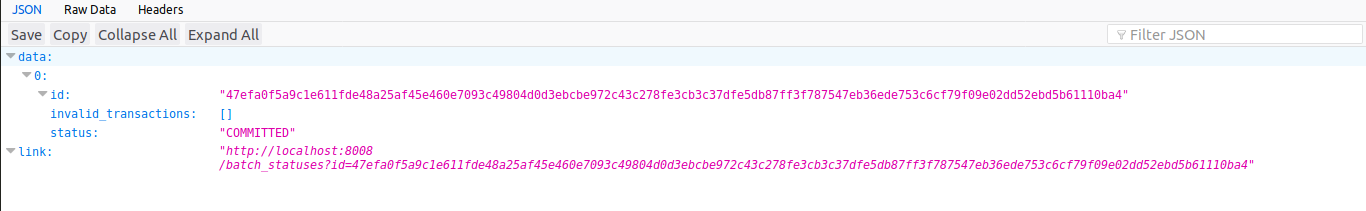
\includegraphics[width=\textwidth]{Issue-Certificate-Status}
	\caption{Status of Transaction \#1.}
	\label{fig:issue-certificate-status}
\end{figure}

\subsection{Viewing a Certificate}
\label{sec:impl-view}

Furthermore, now that our certificate has been issued, we want to be able to see the contents of it. Let's assume we are now impersonating the recipient of the certificate. We would run the \texttt{cert-viewer} script with our secret keys, in able to view the certificate's contents. We demonstrate this in Listing \ref{listing:view-results}.

\begin{listing}[ht]
	\begin{minted}[
frame=lines,
framesep=2mm,
baselinestretch=1.2,
fontsize=\footnotesize,
linenos,
breaklines
]{sh}
$ ./cert-viewer --certificate 2136718e-d4cb-4cb2-b324-936444cf33bd --secret-dsa fff1224e60ee00f6580c3b303b7682f2af601b5180097216aeb18e15eff2e72c --sec
ret-rsa ../keys/recipient.keys/rsa/recipient
Generating Addresses...[OK]
Fetching Data...[OK]
Attempt 1...[Error]
Attempt 2...[OK]

ID: 2136718e-d4cb-4cb2-b324-936444cf33bd
Issuer: 03112e85ea835a6f445c8195f99e64f9677127d12dabcdf43422c9f3cb52aeeb8f
Recipient: 03a1b6863f84cd6b17597e99a09d818a6cd992007136fceed9d3ad93fa7180d32c
Issued @ 2018-10-01 19:32:07.554541
Status: Active


\end{minted}
	\caption{Results of Executing \texttt{cert-viewer} \#1.}
	\label{listing:view-results}
\end{listing}

As we demonstrate in Listing \ref{listing:view-results}, and present in Chapter \ref{chap:design}, a user of \texttt{Protego}, with the appropriate permissions is able to see in full the contents of the certificate. In this case, since we are impersonating the recipient of the certificate it only makes sense that we are able to view its contents. In the results, \emph{Attempt 1} and \emph{Attempt 2} represent the attempts at decrypting the symmetric key with the RSA secret key. No transaction is submitted in this activity such that there's no need to make any validation within the blockchain.

\subsection{Granting Access}
\label{sec:impl-grant-ac}

Let us now assume the following scenario: a recruiter approaches the recipient of the certificate, in the hopes of hiring the recipient. The recruiter wishes to verify the qualifications that the recipient claims to have. In that context, the recruiter will share the public keys, both for RSA and DSA, so that the recipient can provide the recruiter with access to the certificate stored in the blockchain. We demonstrate the results of this in Listing \ref{listing:grant-ac-results}. We achieve the desired results by running the `manager' script with the appropriate parameters.

\begin{listing}[ht]
	\begin{minted}[
frame=lines,
framesep=2mm,
baselinestretch=1.2,
fontsize=\footnotesize,
linenos,
breaklines
]{sh}
$ ./manager -c 2136718e-d4cb-4cb2-b324-936444cf33bd  --subject-dsa 036933186998989510747d4f75860e163f7e00454a33bef557ec0c96bd4b4ce389 --subject-rsa ..
/keys/recruiter.keys/rsa/recruiter.pub --secret-dsa fff1224e60ee00f6580c3b303b7682f2af601b5180097216aeb18e15eff2e72c --secret-rsa ../keys/recipient.ke
ys/rsa/recipient

Generating Addresses...[OK]
Fetching Data...[OK]
Attempt 1...[Error]
Attempt 2...[OK]
Generating Payload...[OK]
Creating Transaction...[OK]
Creating Batch...[OK]
Submitting Request...[OK]

Status:
http://localhost:8008/batch_statuses?id=046d0e13fb5bacafbeed3b8b353e44d6b6a9f1c4a6e9210d934870dee6c5c228474
7fd62cb8035317bc98eb3a9b3067a8eb00558b5d6e69de7360494357a8bf3
\end{minted}
	\caption{Results of Granting Access with \texttt{manager}.}
	\label{listing:grant-ac-results}
\end{listing}

Similary to what happens when issuing a certificate, the user must confirm that the transaction has been accepted. We demonstrate this in Figure \ref{fig:grant-ac-status}.

\begin{figure}[htb]
	\centering
	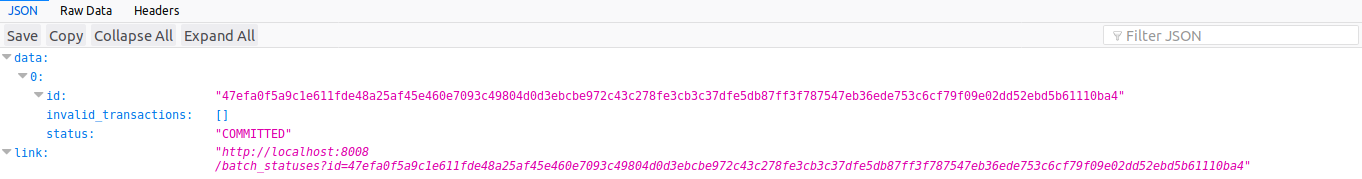
\includegraphics[width=\textwidth]{Grant-AC-Status}
	\caption{Status of Transaction \#2.}
	\label{fig:grant-ac-status}
\end{figure}

After confirming that the permission has been granted, the recipient can now inform the recruiter what certificate address it should query for - in this case "2136718e-d4cb-4cb2-b324-936444cf33bd". We demonstrate this in Listing \ref{listing:view-recruiter-grant-results}, which uses the same components of the previous example, where we viewed the contents of the certificate. It is interesting to confirm that the certificate in question has, now, an additional iteration at decrypting the certificate - \emph{Attempt 3}. 

\begin{listing}[ht]
	\begin{minted}[
frame=lines,
framesep=2mm,
baselinestretch=1.2,
fontsize=\footnotesize,
linenos,
breaklines
]{sh}
$ ./cert-viewer --certificate 2136718e-d4cb-4cb2-b324-936444cf33bd --secret-dsa 964fb14dad3764286e0620710d02eaea59aa04529bde19447f6ad3d6485a773c --sec
ret-rsa ../keys/recruiter.keys/rsa/recruiter
Generating Addresses...[OK]
Fetching Data...[OK]
Attempt 1...[Error]
Attempt 2...[Error]
Attempt 3...[OK]

ID: 2136718e-d4cb-4cb2-b324-936444cf33bd
Issuer: 03112e85ea835a6f445c8195f99e64f9677127d12dabcdf43422c9f3cb52aeeb8f
Recipient: 03a1b6863f84cd6b17597e99a09d818a6cd992007136fceed9d3ad93fa7180d32c
Issued @ 2018-10-01 19:32:07.554541
Status: Active

\end{minted}
	\caption{Results of Executing \texttt{cert-viewer} \#2.}
	\label{listing:view-recruiter-grant-results}
\end{listing}

\subsection{Revoking Access}
\label{sec:impl-revoke-ac}

Let us now assume that, for some reason, the recruiter shall no longer have access to this certificate. The recipient is able to remove such permission from the certificate's permission list. To do this, it must submit a transaction through \texttt{Protego} in order to remove the permission. We demonstrate this activity in Listing \ref{listing:revoke-ac-results}, in which we run \texttt{manager} with the appropriate \texttt{-r} flag.

\begin{listing}[ht]
	\begin{minted}[
frame=lines,
framesep=2mm,
baselinestretch=1.2,
fontsize=\footnotesize,
linenos,
breaklines
]{sh}
$ ./manager -r -c 2136718e-d4cb-4cb2-b324-936444cf33bd  --subject-dsa 036933186998989510747d4f75860e163f7e00454a33bef557ec0c96bd4b4ce389 --subject-rsa
../keys/recruiter.keys/rsa/recruiter.pub --secret-dsa fff1224e60ee00f6580c3b303b7682f2af601b5180097216aeb18e15eff2e72c --secret-rsa ../keys/recipient
.keys/rsa/recipient

Generating Addresses...[OK]
Fetching Data...[OK]
Attempt 1...[Error]
Attempt 2...[OK]
Generating Payload...[OK]
Creating Transaction...[OK]
Creating Batch...[OK]
Submitting Request...[OK]

Status:
http://localhost:8008/batch_statuses?id=230706d8ad7897c563166ef3bf3853018bb4cf6f3e73dc5d681cbb227cf3644224d
e247aee8c8173126aa9bef1dc56e1abbbd0174d56d1080bc412f0573be4dc
\end{minted}
	\caption{Results of Revoking Access with \texttt{manager}.}
	\label{listing:revoke-ac-results}
\end{listing}

As previously, the recipient can confirm the revokation of the access by checking, through a browser that the transaction has been committed. We demonstrate this in Figure \ref{fig:revoke-ac-status}.

\begin{figure}[htb]
	\centering
	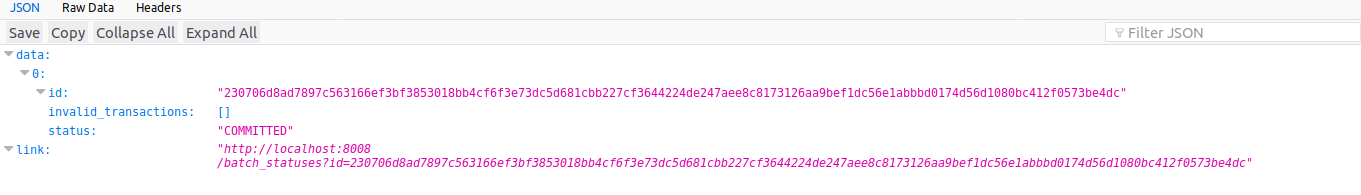
\includegraphics[width=\textwidth]{Revoke-AC-Status}
	\caption{Status of Transaction \#3.}
	\label{fig:revoke-ac-status}
\end{figure}

In this case, contrary to what occurs in Listing \ref{listing:view-recruiter-grant-results}, if the recruiter tries to access the data, after access has been revoked, he will be met with an error. We demonstrate this in Listing \ref{listing:view-recruiter-revoke-results}. It is interesting to note, once again, that the \emph{number} of permissions has decreased, due to the revocation of the recruiter's permission.

\begin{listing}[ht]
	\begin{minted}[
frame=lines,
framesep=2mm,
baselinestretch=1.2,
fontsize=\footnotesize,
linenos,
breaklines
]{sh}
$ ./cert-viewer --certificate 2136718e-d4cb-4cb2-b324-936444cf33bd --secret-dsa 964fb14dad3764286e0620710d02eaea59aa04529bde19447f6ad3d6485a773c --secret-rsa ../keys/recruiter.keys/rsa/recruiter
Generating Addresses...[OK]
Fetching Data...[OK]
Attempt 1...[Error]
Attempt 2...[Error]
error: you do not have permission to access this certificate
\end{minted}
	\caption{Results of Executing \texttt{cert-viewer} \#2.}
	\label{listing:view-recruiter-revoke-results}
\end{listing}

\subsection{Revoking a Certificate}
\label{sec:impl-revoke}

Finally, to conclude our proof-of-concept, let us imagine that the issuer wishes to revoke the certificate it has granted to the recipient, due to, for example, a misconduct condemnation. The recruiter would do this by executing the \texttt{cert-revoker} script which would submit a transaction to the blockchain, revoking the certificate. We demonstrate this in Listing \ref{listing:revoke-results}.

\begin{listing}[ht]
	\begin{minted}[
frame=lines,
framesep=2mm,
baselinestretch=1.2,
fontsize=\footnotesize,
linenos,
breaklines
]{sh}
$ ./cert-revoker -c 2136718e-d4cb-4cb2-b324-936444cf33bd --secret-dsa 396b644103a8fbdebcd17aff319e7b7fc60d879282b54a7a56d8ca53c61d3876 --secret-rsa ..
/keys/issuer.keys/rsa/issuer

Generating Addresses...[OK]
Fetching Data...[OK]
Attempt 1...[OK]
Generating Payload...[OK]
Creating Transaction...[OK]
Creating Batch...[OK]
Submitting Request...[OK]

Status:
http://localhost:8008/batch_statuses?id=cbec918ba2b42601e8d8b25158bde676150ce4e0553897b5c21324f34200200b4c4
2f74c2a1833d96eae1401330f3406766b41eb950e61bc1aeb6e852c11d28b

\end{minted}
	\caption{Results of Executing \texttt{cert-revoker}.}
	\label{listing:revoke-results}
\end{listing}

As with previous submission of transactions, the user should confirm that the transaction has been committed, by accessing the returned URL. We demonstrate this in Figure \ref{fig:revoke-status}.

\begin{figure}[htb]
	\centering
	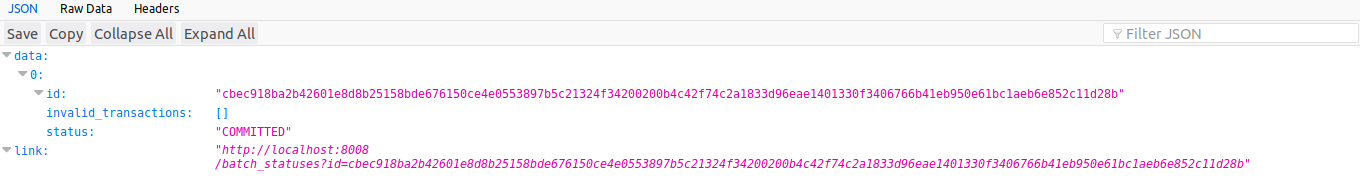
\includegraphics[width=\textwidth]{Revoke-Certificate-Status}
	\caption{Status of Transaction \#4.}
	\label{fig:revoke-status}
\end{figure}

Nonetheless, as explained previously, the certificate is not deleted. If the recipient wishes to view the certificate's contents, it would be able to. The only difference is that the certificate is now irrevocably revoked and will return as such. We demonstrate this in Listing \ref{listing:view-revoke-results}, produced by executing the \texttt{cert-viewer} script, which displays the \texttt{Status} as "Revoked".

\begin{listing}[ht]
	\begin{minted}[
frame=lines,
framesep=2mm,
baselinestretch=1.2,
fontsize=\footnotesize,
linenos,
breaklines
]{sh}
$ ./cert-viewer --certificate 2136718e-d4cb-4cb2-b324-936444cf33bd --secret-dsa fff1224e60ee00f6580c3b303b7682f2af601b5180097216aeb18e15eff2e72c --secret-rsa ../keys/recipient.keys/rsa/recipient
Generating Addresses...[OK]
Fetching Data...[OK]
Attempt 1...[Error]
Attempt 2...[OK]

ID: 2136718e-d4cb-4cb2-b324-936444cf33bd
Issuer: 03112e85ea835a6f445c8195f99e64f9677127d12dabcdf43422c9f3cb52aeeb8f
Recipient: 03a1b6863f84cd6b17597e99a09d818a6cd992007136fceed9d3ad93fa7180d32c
Issued @ 2018-10-01 19:32:07.554541
Status: Revoked

\end{minted}
	\caption{Results of Executing \texttt{cert-viewer} \#3.}
	\label{listing:view-revoke-results}
\end{listing}

\section{Summary}

\textcolor{red}{TODO}
